% The generic preamble
\documentclass[10pt,letterpaper,fleqn,titlepage]{article}

% Define packages to use
\usepackage{natbib}
\usepackage[dvips]{graphicx,color}
\usepackage{amsmath,amssymb}
\usepackage{bm}
\usepackage{caption}
\usepackage{xr}
\usepackage{ifthen}
\usepackage[dvipdfm,colorlinks,linkcolor=blue,citecolor=blue,urlcolor=blue]{hyperref}
\usepackage{fancybox}
\usepackage{textcomp}
\usepackage{alltt}
%\usepackage{floatflt}
%\usepackage{svn}


% Redefine default page
\setlength{\textheight}{9in}  % 1" above and below
\setlength{\textwidth}{6.75in}   % 0.5" left and right
\setlength{\oddsidemargin}{-0.25in}

% Redefine default paragraph
\setlength{\parindent}{0pt}
\setlength{\parskip}{1ex plus 0.5ex minus 0.2ex}

% Define caption width and default fonts
\setlength{\captionmargin}{0.5in}
\renewcommand{\captionfont}{\sffamily}
\renewcommand{\captionlabelfont}{\bfseries\sffamily}

% Define commands for super- and subscript in text mode
\newcommand{\superscript}[1]{\ensuremath{^\textrm{#1}}}
\newcommand{\subscript}[1]{\ensuremath{_\textrm{#1}}}

% Derived commands
\newcommand{\invcm}{\textrm{cm\superscript{-1}}}
\newcommand{\micron}{\ensuremath{\mu\textrm{m}}}

\newcommand{\df}{\ensuremath{\delta f}}
\newcommand{\Df}{\ensuremath{\Delta f}}
\newcommand{\dx}{\ensuremath{\delta x}}
\newcommand{\Dx}{\ensuremath{X_{max}}}
\newcommand{\Xeff}{\ensuremath{X_{eff}}}

\newcommand{\water}{\textrm{H\subscript{2}O}}
\newcommand{\carbondioxide}{\textrm{CO\subscript{2}}}
\newcommand{\ozone}{\textrm{O\subscript{3}}}

\newcommand{\taup}[1]{\ensuremath{\tau_{#1}}}
\newcommand{\efftaup}[1]{\ensuremath{\tau_{#1}^{*}}}

\newcommand{\textbfm}[1]{\boldmath\ensuremath{#1}\unboldmath}

\newcommand{\rb}[1]{\raisebox{1.5ex}[0pt]{#1}}

\newcommand{\f}[1]{\texttt{#1}}

% Define how equations are numbered
\numberwithin{equation}{section}
\numberwithin{figure}{section}
\numberwithin{table}{section}

% Define a command for title page author email footnote
\newcommand{\email}[1]
{%
  \renewcommand{\thefootnote}{\alph{footnote}}%
  \footnote{#1}
  \renewcommand{\thefootnote}{\arabic{footnote}}
}

% Define a command to print the Office Note subheading
\newcommand{\notesubheading}[1]
{%
  \ifthenelse{\equal{#1}{}}{}
  { {\Large\bfseries Office Note #1\par}%
    {\scriptsize \sc This is an unreviewed manuscript, primarily intended for informal}\\ 
    {\scriptsize \sc exchange of information among JCSDA researchers\par}%
  }
}

% Redefine the maketitle macro
\makeatletter
\def\docseries#1{\def\@docseries{#1}}
\def\docnumber#1{\def\@docnumber{#1}}
\renewcommand{\maketitle}
{%
  \thispagestyle{empty}
  \vspace*{1in}
  \begin{center}%
     \sffamily
     {\huge\bfseries Joint Center for Satellite Data Assimilation\par}%
     \notesubheading{\@docnumber}
  \end{center}
  \begin{flushleft}%
     \sffamily
     \vspace*{0.5in}
     {\Large\bfseries\ifthenelse{\equal{\@docseries}{}}{}{\@docseries: }\@title\par}%
     \medskip
     {\large\@author\par}%
     \medskip
     {\large\@date\par}%
     \bigskip\hrule\vspace*{2pc}%
  \end{flushleft}%
  \newpage
  \setcounter{footnote}{0}
}
\makeatother
\docseries{}
\docnumber{}


% Define a command for a DRAFT watermark
\usepackage{eso-pic}
\newcommand{\draftwatermark}
{
  \AddToShipoutPicture{%
    \definecolor{lightgray}{gray}{.85}
    \setlength{\unitlength}{1in}
    \put(2.5,3.5){%
      \rotatebox{45}{%
        \resizebox{4in}{1in}{%
          \textsf{\textcolor{lightgray}{DRAFT}}
        }
      }
    }
  }
}




% Include files
\includeonly{SRF_Data_Plots.app}

% Subversion keywords
\SVN $Date$
\SVN $Revision$

% Title info
\title{HIRS Sounder Spectral Response Function Processing}
\author{Paul van Delst\email{paul.vandelst@noaa.gov}\\NCEP/EMC/IMSG}
\date{\SVNDate ; rev\SVNRevision}
\docnumber{4}
\docseries{CRTM}


%-------------------------------------------------------------------------------
%                            Ze document begins...
%-------------------------------------------------------------------------------
\begin{document}
\maketitle

\draftwatermark

% The front matter
%=================
\thispagestyle{empty}
\vspace*{10cm}
\begin{center}
  {\sffamily\Large\bfseries Change History}
  \begin{table}[htp]
    \centering
    \begin{tabular}{|p{2cm}|p{3cm}|p{8cm}|}
      \hline
      \sffamily\textbf{Date} & \sffamily\textbf{Author} & \sffamily\textbf{Change}\\
      \hline\hline
      2013-12-04 & Paul van Delst & Initial draft/placeholder document. SRF processing is provisional (and for some channels incorrect).\\
      \hline
    \end{tabular}
  \end{table}
\end{center}
\clearpage
\pagestyle{fancy}
\fancyhead[LE,RO]{\sffamily \rightmark}
\fancyhead[LO,RE]{\sffamily \leftmark}
\pagenumbering{arabic}
\setcounter{page}{1}


% The main matter
%================

\section{Introduction}
%=====================
This document describes the pre-processing applied to the HIRS sounder instrument spectral response functions (SRFs), obtained from \cite{HIRS_SRF_Data}, to prepare for use in the CRTM processing chain. The SRFs are used to generate channel central frequencies, as well as in the convolution of monochromatic quantities such as Planck radiances or line-by-line (LBL) model generated transmittances to produce such things as polychromatic correction coefficients and instrument resolution transmittances. The latter, for a diverse set of atmospheric profiles, are then regressed against a set of predictors to produce the fast transmittance model coefficients used by the CRTM.


\subsection{Computation of the channel central frequency}
%--------------------------------------------------------
The computed channel central frequencies, $\nu_0$, are the first moments of the defined SRF, $\phi(\nu)$,
\begin{equation}
  \nu_0 = \frac{\displaystyle\int{\nu\:\phi(\nu)\ud \nu}}{\displaystyle\int{\phi(\nu)\ud \nu}}
\end{equation}


\subsection{Computation of polychromatic correction coefficients}
%----------------------------------------------------------------
In the CRTM, the conversion of \emph{channel resolution} radiances to brightness temperatures has to take the channel bandwidth into account. For any channel, the regression relation to be solved is

\begin{equation}
  a_0 + a_1T + \ldots = \frac{\displaystyle k_1}{\displaystyle \ln\left[\frac{k_2}{R(T)}+1\right]} = Y(T)
\end{equation}
where
\begin{equation}
  \begin{array}{r@{\;=\;}l}
         T &\mbox{brightness temperature} \\
        a_j&\mbox{regression coefficients} \\
    k_1,k_2&\mbox{Planck coefficients} \\
       R(T)&\mbox{channel radiance} \\
       Y(T)&\mbox{``effective'' brightness temperature}
  \end{array}
\end{equation}
and the channel radiances used to determine the effective temperatures, $Y(T)$, are computed the usual way
\begin{equation}
  R(T) = \frac{\displaystyle\int{B(T,\nu)\:\phi(\nu)\ud \nu}}{\displaystyle\int{\phi(\nu)\ud \nu}}
\end{equation}
The quantity minimised to obtain the $a_j$ coefficients is
\begin{equation}
  \left[ \sum_{j=0}^{M}a_j T_{i} - Y(T_{i}) \right]^2 \quad\mbox{for}\quad T_i = 150K, \ldots, 340K \;\mbox{ in 5K steps.}
\end{equation}
Currently the number of coefficients is fixed at two (i.e. $M=1$).



\newpage
\section{Summary}
%================

The following tables list the computed central frequencies and polychromatic correction coefficients for the various HIRS instruments. Plots of the SRF data for each channel, along with their temperature fit residuals, are shown in appendix \ref{app.srf_data_plots}.

\subsection{TIROS-N HIRS/2}
%--------------------------
\begin{table}[H]
\centering
\begin{tabular}{c *{3}{c r@{.}l}}
  \hline
  \sffamily{Channel} & & \multicolumn{2}{c}{$f_0$} & & \multicolumn{2}{c}{$a_0$ \textsf{(offset)}} & & \multicolumn{2}{c}{$a_1$ \textsf{(slope)}} \\
                     & & \multicolumn{2}{c}{\sffamily{(cm\superscript{-1})}} & & \multicolumn{2}{c}{\sffamily{(K)}} & & \multicolumn{2}{c}{\sffamily{(K/K)}}  \\
  \hline\hline
    1 & &  669&00369 & & -0&00923732 & &  1&00004521 \\
    2 & &  679&35078 & &  0&00271412 & &  0&99998893 \\
    3 & &  690&68743 & &  0&02248614 & &  0&99989840 \\
    4 & &  704&29537 & &  0&02572982 & &  0&99988616 \\
    5 & &  716&19278 & &  0&02337930 & &  0&99989835 \\
    6 & &  732&04576 & &  0&02886629 & &  0&99987720 \\
    7 & &  748&93434 & &  0&03087054 & &  0&99987160 \\
    8 & &  899&67097 & &  0&08475871 & &  0&99970100 \\
    9 & & 1027&33275 & &  0&06438028 & &  0&99979647 \\
   10 & & 1220&64156 & &  0&19747169 & &  0&99945902 \\
   11 & & 1363&23568 & &  0&09876798 & &  0&99975260 \\
   12 & & 1482&91850 & &  0&33559703 & &  0&99922155 \\
   13 & & 2191&35101 & &  0&02034267 & &  0&99996631 \\
   14 & & 2211&95954 & &  0&01948084 & &  0&99996785 \\
   15 & & 2238&50482 & &  0&02532233 & &  0&99995846 \\
   16 & & 2273&23037 & &  0&05457454 & &  0&99991058 \\
   17 & & 2359&19205 & &  0&02340764 & &  0&99996349 \\
   18 & & 2510&42390 & &  0&06837237 & &  0&99989741 \\
   19 & & 2660&57548 & &  0&35996417 & &  0&99948667 \\
    \hline
  \end{tabular}
  \caption{The computed TIROS-N HIRS/2 channel central frequencies and polychromatic correction coefficients.}
  \label{tab:hirs2_tirosn_results}
\end{table}

\subsection{NOAA-6 HIRS/2}
%--------------------------
\begin{table}[H]
\centering
\begin{tabular}{c *{3}{c r@{.}l}}
  \hline
  \sffamily{Channel} & & \multicolumn{2}{c}{$f_0$} & & \multicolumn{2}{c}{$a_0$ \textsf{(offset)}} & & \multicolumn{2}{c}{$a_1$ \textsf{(slope)}} \\
                     & & \multicolumn{2}{c}{\sffamily{(cm\superscript{-1})}} & & \multicolumn{2}{c}{\sffamily{(K)}} & & \multicolumn{2}{c}{\sffamily{(K/K)}}  \\
  \hline\hline
    1 & &  667&93834 & &  0&00662149 & &  0&99996895 \\
    2 & &  679&34430 & &  0&01559832 & &  0&99992829 \\
    3 & &  690&01129 & &  0&02343187 & &  0&99989401 \\
    4 & &  704&61735 & &  0&02684075 & &  0&99988131 \\
    5 & &  717&74366 & &  0&02524011 & &  0&99989048 \\
    6 & &  732&30906 & &  0&02911634 & &  0&99987617 \\
    7 & &  749&15365 & &  0&03070533 & &  0&99987230 \\
    8 & &  899&96315 & &  0&07119913 & &  0&99974864 \\
    9 & & 1027&58503 & &  0&06128593 & &  0&99980637 \\
   10 & & 1222&63586 & &  0&19631187 & &  0&99946273 \\
   11 & & 1368&53212 & &  0&09792542 & &  0&99975617 \\
   12 & & 1481&19457 & &  0&35719997 & &  0&99916982 \\
   13 & & 2190&47345 & &  0&01771093 & &  0&99997050 \\
   14 & & 2210&86567 & &  0&01845728 & &  0&99996950 \\
   15 & & 2237&64393 & &  0&02292779 & &  0&99996243 \\
   16 & & 2269&66379 & &  0&01898822 & &  0&99996931 \\
   17 & & 2360&93807 & &  0&02134004 & &  0&99996664 \\
   18 & & 2515&25792 & &  0&05857233 & &  0&99991355 \\
   19 & & 2650&00347 & &  0&36000753 & &  0&99949027 \\
    \hline
  \end{tabular}
  \caption{The computed NOAA-6 HIRS/2 channel central frequencies and polychromatic correction coefficients.}
  \label{tab:hirs2_n06_results}
\end{table}

\subsection{NOAA-7 HIRS/2}
%--------------------------
\begin{table}[H]
\centering
\begin{tabular}{c *{3}{c r@{.}l}}
  \hline
  \sffamily{Channel} & & \multicolumn{2}{c}{$f_0$} & & \multicolumn{2}{c}{$a_0$ \textsf{(offset)}} & & \multicolumn{2}{c}{$a_1$ \textsf{(slope)}} \\
                     & & \multicolumn{2}{c}{\sffamily{(cm\superscript{-1})}} & & \multicolumn{2}{c}{\sffamily{(K)}} & & \multicolumn{2}{c}{\sffamily{(K/K)}}  \\
  \hline\hline
    1 & &  667&98792 & &  0&00485698 & &  0&99997723 \\
    2 & &  678&82468 & &  0&01422713 & &  0&99993454 \\
    3 & &  691&79596 & &  0&02430200 & &  0&99989039 \\
    4 & &  704&61341 & &  0&02196407 & &  0&99990288 \\
    5 & &  717&23339 & &  0&02452316 & &  0&99989355 \\
    6 & &  733&76927 & &  0&02974967 & &  0&99987373 \\
    7 & &  749&63339 & &  0&03067002 & &  0&99987253 \\
    8 & &  897&36771 & &  0&07218344 & &  0&99974456 \\
    9 & & 1026&04741 & &  0&06262734 & &  0&99980177 \\
   10 & & 1221&49618 & &  0&19022094 & &  0&99947928 \\
   11 & & 1363&54243 & &  0&09000901 & &  0&99977503 \\
   12 & & 1484&48108 & &  0&34519980 & &  0&99919495 \\
   13 & & 2182&28126 & &  0&02504756 & &  0&99995798 \\
   14 & & 2206&92411 & &  0&02260762 & &  0&99996225 \\
   15 & & 2239&94788 & &  0&02273616 & &  0&99996280 \\
   16 & & 2270&84894 & &  0&02117195 & &  0&99996580 \\
   17 & & 2357&15930 & &  0&02125193 & &  0&99996692 \\
   18 & & 2513&99839 & &  0&05779117 & &  0&99991536 \\
   19 & & 2652&77211 & &  0&35195725 & &  0&99950420 \\
    \hline
  \end{tabular}
  \caption{The computed NOAA-7 HIRS/2 channel central frequencies and polychromatic correction coefficients.}
  \label{tab:hirs2_n07_results}
\end{table}

\subsection{NOAA-8 HIRS/2}
%--------------------------
\begin{table}[H]
\centering
\begin{tabular}{c *{3}{c r@{.}l}}
  \hline
  \sffamily{Channel} & & \multicolumn{2}{c}{$f_0$} & & \multicolumn{2}{c}{$a_0$ \textsf{(offset)}} & & \multicolumn{2}{c}{$a_1$ \textsf{(slope)}} \\
                     & & \multicolumn{2}{c}{\sffamily{(cm\superscript{-1})}} & & \multicolumn{2}{c}{\sffamily{(K)}} & & \multicolumn{2}{c}{\sffamily{(K/K)}}  \\
  \hline\hline
    1 & &  667&02163 & &  0&01212857 & &  0&99994287 \\
    2 & &  678&85381 & &  0&01379061 & &  0&99993655 \\
    3 & &  690&31023 & &  0&02500358 & &  0&99988694 \\
    4 & &  703&07833 & &  0&02505266 & &  0&99988899 \\
    5 & &  717&68528 & &  0&02313234 & &  0&99989961 \\
    6 & &  732&14628 & &  0&02923592 & &  0&99987562 \\
    7 & &  748&58013 & &  0&03048574 & &  0&99987315 \\
    8 & &  898&91760 & &  0&07072281 & &  0&99975010 \\
    9 & & 1026&37949 & &  0&06203253 & &  0&99980371 \\
   10 & & 1220&95358 & &  0&19913901 & &  0&99945499 \\
   11 & & 1366&03782 & &  0&09641010 & &  0&99975948 \\
   12 & & 1483&16453 & &  0&34325293 & &  0&99919893 \\
   13 & & 2188&19619 & &  0&01973960 & &  0&99996711 \\
   14 & & 2210&32088 & &  0&02488076 & &  0&99995873 \\
   15 & & 2238&23905 & &  0&01848736 & &  0&99996973 \\
   16 & & 2271&12011 & &  0&02153473 & &  0&99996519 \\
   17 & & 2357&24778 & &  0&02036284 & &  0&99996833 \\
   18 & & 2514&75382 & &  0&05943786 & &  0&99991259 \\
   19 & & 2656&38245 & &  0&35082731 & &  0&99950410 \\
    \hline
  \end{tabular}
  \caption{The computed NOAA-8 HIRS/2 channel central frequencies and polychromatic correction coefficients.}
  \label{tab:hirs2_n08_results}
\end{table}

\subsection{NOAA-9 HIRS/2}
%--------------------------
\begin{table}[H]
\centering
\begin{tabular}{c *{3}{c r@{.}l}}
  \hline
  \sffamily{Channel} & & \multicolumn{2}{c}{$f_0$} & & \multicolumn{2}{c}{$a_0$ \textsf{(offset)}} & & \multicolumn{2}{c}{$a_1$ \textsf{(slope)}} \\
                     & & \multicolumn{2}{c}{\sffamily{(cm\superscript{-1})}} & & \multicolumn{2}{c}{\sffamily{(K)}} & & \multicolumn{2}{c}{\sffamily{(K/K)}}  \\
  \hline\hline
    1 & &  667&56331 & &  0&00744355 & &  0&99996503 \\
    2 & &  679&79265 & &  0&01414711 & &  0&99993500 \\
    3 & &  691&13954 & &  0&02298467 & &  0&99989624 \\
    4 & &  703&50640 & &  0&02545277 & &  0&99988728 \\
    5 & &  717&21781 & &  0&02343818 & &  0&99989825 \\
    6 & &  732&91686 & &  0&03147818 & &  0&99986626 \\
    7 & &  749&63368 & &  0&02703746 & &  0&99988766 \\
    8 & &  898&17529 & &  0&07179706 & &  0&99974614 \\
    9 & & 1030&41846 & &  0&06195083 & &  0&99980455 \\
   10 & & 1220&13813 & &  0&19079973 & &  0&99947731 \\
   11 & & 1365&99775 & &  0&09152345 & &  0&99977188 \\
   12 & & 1483&39244 & &  0&35688711 & &  0&99917007 \\
   13 & & 2190&69835 & &  0&01948379 & &  0&99996777 \\
   14 & & 2209&68647 & &  0&01982504 & &  0&99996721 \\
   15 & & 2242&88440 & &  0&01887209 & &  0&99996919 \\
   16 & & 2274&44560 & &  0&05464100 & &  0&99991103 \\
   17 & & 2359&85360 & &  0&02218948 & &  0&99996535 \\
   18 & & 2517&14592 & &  0&05713279 & &  0&99991614 \\
   19 & & 2663&45464 & &  0&34085348 & &  0&99951562 \\
    \hline
  \end{tabular}
  \caption{The computed NOAA-9 HIRS/2 channel central frequencies and polychromatic correction coefficients.}
  \label{tab:hirs2_n09_results}
\end{table}

\subsection{NOAA-10 HIRS/2}
%--------------------------
\begin{table}[H]
\centering
\begin{tabular}{c *{3}{c r@{.}l}}
  \hline
  \sffamily{Channel} & & \multicolumn{2}{c}{$f_0$} & & \multicolumn{2}{c}{$a_0$ \textsf{(offset)}} & & \multicolumn{2}{c}{$a_1$ \textsf{(slope)}} \\
                     & & \multicolumn{2}{c}{\sffamily{(cm\superscript{-1})}} & & \multicolumn{2}{c}{\sffamily{(K)}} & & \multicolumn{2}{c}{\sffamily{(K/K)}}  \\
  \hline\hline
    1 & &  667&58865 & &  0&00698109 & &  0&99996717 \\
    2 & &  680&20719 & &  0&01434969 & &  0&99993412 \\
    3 & &  691&31751 & &  0&02444669 & &  0&99988965 \\
    4 & &  704&46111 & &  0&02201163 & &  0&99990263 \\
    5 & &  716&73810 & &  0&02235135 & &  0&99990288 \\
    6 & &  732&95205 & &  0&03012726 & &  0&99987201 \\
    7 & &  750&51345 & &  0&03353722 & &  0&99986079 \\
    8 & &  898&59000 & &  0&07009166 & &  0&99975227 \\
    9 & & 1027&74243 & &  0&06212979 & &  0&99980363 \\
   10 & & 1223&60266 & &  0&20503272 & &  0&99943967 \\
   11 & & 1364&05020 & &  0&09450065 & &  0&99976361 \\
   12 & & 1483&34884 & &  0&34612037 & &  0&99919291 \\
   13 & & 2189&64992 & &  0&02240860 & &  0&99996265 \\
   14 & & 2206&68950 & &  0&02347504 & &  0&99996076 \\
   15 & & 2239&51865 & &  0&02300612 & &  0&99996256 \\
   16 & & 2268&18694 & &  0&02104140 & &  0&99996599 \\
   17 & & 2359&03539 & &  0&01827609 & &  0&99997154 \\
   18 & & 2512&98891 & &  0&05504319 & &  0&99991909 \\
   19 & & 2659&84061 & &  0&32162015 & &  0&99954917 \\
    \hline
  \end{tabular}
  \caption{The computed NOAA-10 HIRS/2 channel central frequencies and polychromatic correction coefficients.}
  \label{tab:hirs2_n10_results}
\end{table}

\subsection{NOAA-11 HIRS/2}
%--------------------------
\begin{table}[H]
\centering
\begin{tabular}{c *{3}{c r@{.}l}}
  \hline
  \sffamily{Channel} & & \multicolumn{2}{c}{$f_0$} & & \multicolumn{2}{c}{$a_0$ \textsf{(offset)}} & & \multicolumn{2}{c}{$a_1$ \textsf{(slope)}} \\
                     & & \multicolumn{2}{c}{\sffamily{(cm\superscript{-1})}} & & \multicolumn{2}{c}{\sffamily{(K)}} & & \multicolumn{2}{c}{\sffamily{(K/K)}}  \\
  \hline\hline
    1 & &  669&00389 & &  0&00973919 & &  0&99995452 \\
    2 & &  678&90739 & &  0&01390429 & &  0&99993604 \\
    3 & &  689&78320 & &  0&02265820 & &  0&99989761 \\
    4 & &  703&37490 & &  0&02230531 & &  0&99990115 \\
    5 & &  716&88823 & &  0&02427639 & &  0&99989455 \\
    6 & &  732&15111 & &  0&02698345 & &  0&99988520 \\
    7 & &  749&44747 & &  0&02566370 & &  0&99989330 \\
    8 & &  900&46337 & &  0&07218044 & &  0&99974534 \\
    9 & & 1031&17441 & &  0&06759003 & &  0&99978698 \\
   10 & &  795&85211 & &  0&02710461 & &  0&99989351 \\
   11 & & 1361&38018 & &  0&09195560 & &  0&99976969 \\
   12 & & 1479&96983 & &  0&29107282 & &  0&99932387 \\
   13 & & 2190&04047 & &  0&02411765 & &  0&99996010 \\
   14 & & 2209&72304 & &  0&01905652 & &  0&99996855 \\
   15 & & 2239&32395 & &  0&02092403 & &  0&99996581 \\
   16 & & 2267&95019 & &  0&01871699 & &  0&99996978 \\
   17 & & 2416&53905 & &  0&02864586 & &  0&99995643 \\
   18 & & 2511&99170 & &  0&05025259 & &  0&99992526 \\
   19 & & 2664&32646 & &  0&33607137 & &  0&99952821 \\
    \hline
  \end{tabular}
  \caption{The computed NOAA-11 HIRS/2 channel central frequencies and polychromatic correction coefficients.}
  \label{tab:hirs2_n11_results}
\end{table}

\subsection{NOAA-12 HIRS/2}
%--------------------------
\begin{table}[H]
\centering
\begin{tabular}{c *{3}{c r@{.}l}}
  \hline
  \sffamily{Channel} & & \multicolumn{2}{c}{$f_0$} & & \multicolumn{2}{c}{$a_0$ \textsf{(offset)}} & & \multicolumn{2}{c}{$a_1$ \textsf{(slope)}} \\
                     & & \multicolumn{2}{c}{\sffamily{(cm\superscript{-1})}} & & \multicolumn{2}{c}{\sffamily{(K)}} & & \multicolumn{2}{c}{\sffamily{(K/K)}}  \\
  \hline\hline
    1 & &  667&59420 & &  0&00877320 & &  0&99995878 \\
    2 & &  680&21476 & &  0&01498208 & &  0&99993123 \\
    3 & &  690&04005 & &  0&02416464 & &  0&99989070 \\
    4 & &  704&21419 & &  0&02448506 & &  0&99989166 \\
    5 & &  716&33938 & &  0&02528264 & &  0&99989011 \\
    6 & &  732&29263 & &  0&03404338 & &  0&99985553 \\
    7 & &  751&79424 & &  0&03157162 & &  0&99986917 \\
    8 & &  898&71820 & &  0&07045174 & &  0&99975100 \\
    9 & & 1025&57077 & &  0&06338402 & &  0&99979930 \\
   10 & & 1221&25649 & &  0&19953683 & &  0&99945418 \\
   11 & & 1367&65598 & &  0&10703164 & &  0&99973319 \\
   12 & & 1480&60734 & &  0&35988769 & &  0&99915898 \\
   13 & & 2188&43696 & &  0&02139835 & &  0&99996415 \\
   14 & & 2210&60213 & &  0&01822658 & &  0&99996988 \\
   15 & & 2238&50985 & &  0&02308333 & &  0&99996241 \\
   16 & & 2267&69100 & &  0&02292141 & &  0&99996295 \\
   17 & & 2361&62268 & &  0&02065081 & &  0&99996761 \\
   18 & & 2514&66550 & &  0&05946952 & &  0&99991252 \\
   19 & & 2653&59734 & &  0&35254713 & &  0&99949984 \\
    \hline
  \end{tabular}
  \caption{The computed NOAA-12 HIRS/2 channel central frequencies and polychromatic correction coefficients.}
  \label{tab:hirs2_n12_results}
\end{table}

\subsection{NOAA-14 HIRS/2}
%--------------------------
\begin{table}[H]
\centering
\begin{tabular}{c *{3}{c r@{.}l}}
  \hline
  \sffamily{Channel} & & \multicolumn{2}{c}{$f_0$} & & \multicolumn{2}{c}{$a_0$ \textsf{(offset)}} & & \multicolumn{2}{c}{$a_1$ \textsf{(slope)}} \\
                     & & \multicolumn{2}{c}{\sffamily{(cm\superscript{-1})}} & & \multicolumn{2}{c}{\sffamily{(K)}} & & \multicolumn{2}{c}{\sffamily{(K/K)}}  \\
  \hline\hline
    1 & &  668&90520 & &  0&00321490 & &  0&99998497 \\
    2 & &  679&42175 & &  0&01352708 & &  0&99993781 \\
    3 & &  689&64245 & &  0&01344424 & &  0&99993917 \\
    4 & &  703&67513 & &  0&02218286 & &  0&99990177 \\
    5 & &  714&68542 & &  0&02196621 & &  0&99990425 \\
    6 & &  732&27586 & &  0&02558126 & &  0&99989121 \\
    7 & &  749&67558 & &  0&02646577 & &  0&99989001 \\
    8 & &  898&65766 & &  0&06916221 & &  0&99975556 \\
    9 & & 1028&42213 & &  0&06125456 & &  0&99980666 \\
   10 & &  796&08210 & &  0&02916754 & &  0&99988545 \\
   11 & & 1361&25845 & &  0&09289896 & &  0&99976729 \\
   12 & & 1481&02790 & &  0&28288137 & &  0&99934318 \\
   13 & & 2191&31478 & &  0&02103657 & &  0&99996505 \\
   14 & & 2207&34656 & &  0&01912939 & &  0&99996839 \\
   15 & & 2236&30677 & &  0&02101985 & &  0&99996560 \\
   16 & & 2268&15972 & &  0&01849859 & &  0&99997016 \\
   17 & & 2420&38168 & &  0&02889436 & &  0&99995608 \\
   18 & & 2512&27243 & &  0&04480396 & &  0&99993382 \\
   19 & & 2648&34309 & &  0&32858068 & &  0&99953777 \\
    \hline
  \end{tabular}
  \caption{The computed NOAA-14 HIRS/2 channel central frequencies and polychromatic correction coefficients.}
  \label{tab:hirs2_n14_results}
\end{table}

\subsection{NOAA-15 HIRS/3}
%--------------------------
\begin{table}[H]
\centering
\begin{tabular}{c *{3}{c r@{.}l}}
  \hline
  \sffamily{Channel} & & \multicolumn{2}{c}{$f_0$} & & \multicolumn{2}{c}{$a_0$ \textsf{(offset)}} & & \multicolumn{2}{c}{$a_1$ \textsf{(slope)}} \\
                     & & \multicolumn{2}{c}{\sffamily{(cm\superscript{-1})}} & & \multicolumn{2}{c}{\sffamily{(K)}} & & \multicolumn{2}{c}{\sffamily{(K/K)}}  \\
  \hline\hline
    1 & &  669&12706 & &  0&00228585 & &  0&99998931 \\
    2 & &  678&76192 & &  0&01159816 & &  0&99994661 \\
    3 & &  690&42875 & &  0&01883989 & &  0&99991482 \\
    4 & &  703&14608 & &  0&01788170 & &  0&99992076 \\
    5 & &  715&92730 & &  0&02388918 & &  0&99989608 \\
    6 & &  731&74268 & &  0&02038723 & &  0&99991320 \\
    7 & &  747&66174 & &  0&02691952 & &  0&99988778 \\
    8 & &  897&36441 & &  0&09661237 & &  0&99965817 \\
    9 & & 1032&10857 & &  0&04772265 & &  0&99984975 \\
   10 & &  801&10560 & &  0&01655523 & &  0&99993531 \\
   11 & & 1362&43734 & &  0&07679643 & &  0&99980751 \\
   12 & & 1529&82496 & &  0&10582079 & &  0&99976038 \\
   13 & & 2188&19324 & &  0&02481033 & &  0&99995893 \\
   14 & & 2209&93866 & &  0&01931216 & &  0&99996809 \\
   15 & & 2235&28094 & &  0&01940503 & &  0&99996825 \\
   16 & & 2241&98591 & &  0&02281718 & &  0&99996269 \\
   17 & & 2418&97679 & &  0&03364566 & &  0&99994885 \\
   18 & & 2518&79714 & &  0&04719649 & &  0&99993104 \\
   19 & & 2657&26231 & &  0&30057797 & &  0&99958090 \\
    \hline
  \end{tabular}
  \caption{The computed NOAA-15 HIRS/3 channel central frequencies and polychromatic correction coefficients.}
  \label{tab:hirs3_n15_results}
\end{table}

\subsection{NOAA-16 HIRS/3}
%--------------------------
\begin{table}[H]
\centering
\begin{tabular}{c *{3}{c r@{.}l}}
  \hline
  \sffamily{Channel} & & \multicolumn{2}{c}{$f_0$} & & \multicolumn{2}{c}{$a_0$ \textsf{(offset)}} & & \multicolumn{2}{c}{$a_1$ \textsf{(slope)}} \\
                     & & \multicolumn{2}{c}{\sffamily{(cm\superscript{-1})}} & & \multicolumn{2}{c}{\sffamily{(K)}} & & \multicolumn{2}{c}{\sffamily{(K/K)}}  \\
  \hline\hline
    1 & &  669&73963 & &  0&00222859 & &  0&99998959 \\
    2 & &  679&83803 & &  0&01267964 & &  0&99994173 \\
    3 & &  691&21067 & &  0&01919118 & &  0&99991334 \\
    4 & &  701&86371 & &  0&01773344 & &  0&99992124 \\
    5 & &  716&56530 & &  0&02430002 & &  0&99989438 \\
    6 & &  731&33692 & &  0&02005149 & &  0&99991458 \\
    7 & &  749&78169 & &  0&02742696 & &  0&99988602 \\
    8 & &  897&85210 & &  0&09902897 & &  0&99964984 \\
    9 & & 1032&37077 & &  0&04758227 & &  0&99985025 \\
   10 & &  803&52759 & &  0&01648956 & &  0&99993575 \\
   11 & & 1364&27011 & &  0&07434557 & &  0&99981392 \\
   12 & & 1526&89115 & &  0&11064076 & &  0&99974878 \\
   13 & & 2186&96332 & &  0&02489423 & &  0&99995877 \\
   14 & & 2206&50974 & &  0&01876208 & &  0&99996895 \\
   15 & & 2233&29732 & &  0&02011997 & &  0&99996701 \\
   16 & & 2242&85314 & &  0&02219385 & &  0&99996374 \\
   17 & & 2417&94918 & &  0&03573421 & &  0&99994568 \\
   18 & & 2517&81382 & &  0&04772569 & &  0&99993017 \\
   19 & & 2666&25955 & &  0&30635248 & &  0&99957305 \\
    \hline
  \end{tabular}
  \caption{The computed NOAA-16 HIRS/3 channel central frequencies and polychromatic correction coefficients.}
  \label{tab:hirs3_n16_results}
\end{table}

\subsection{NOAA-17 HIRS/3}
%--------------------------
\begin{table}[H]
\centering
\begin{tabular}{c *{3}{c r@{.}l}}
  \hline
  \sffamily{Channel} & & \multicolumn{2}{c}{$f_0$} & & \multicolumn{2}{c}{$a_0$ \textsf{(offset)}} & & \multicolumn{2}{c}{$a_1$ \textsf{(slope)}} \\
                     & & \multicolumn{2}{c}{\sffamily{(cm\superscript{-1})}} & & \multicolumn{2}{c}{\sffamily{(K)}} & & \multicolumn{2}{c}{\sffamily{(K/K)}}  \\
  \hline\hline
    1 & &  668&88631 & &  0&00248668 & &  0&99998836 \\
    2 & &  680&01229 & &  0&01235850 & &  0&99994322 \\
    3 & &  691&43725 & &  0&01882801 & &  0&99991501 \\
    4 & &  702&72823 & &  0&01774469 & &  0&99992132 \\
    5 & &  715&73502 & &  0&02567464 & &  0&99988829 \\
    6 & &  731&82891 & &  0&02133805 & &  0&99990916 \\
    7 & &  748&03963 & &  0&02759057 & &  0&99988507 \\
    8 & &  899&90193 & &  0&10031548 & &  0&99964590 \\
    9 & & 1029&15808 & &  0&04001131 & &  0&99987366 \\
   10 & &  801&50365 & &  0&01816129 & &  0&99992908 \\
   11 & & 1365&22786 & &  0&07139971 & &  0&99982148 \\
   12 & & 1527&76654 & &  0&10913771 & &  0&99975239 \\
   13 & & 2185&58518 & &  0&02541230 & &  0&99995798 \\
   14 & & 2210&97945 & &  0&01954997 & &  0&99996768 \\
   15 & & 2232&98949 & &  0&02077150 & &  0&99996593 \\
   16 & & 2240&37607 & &  0&02187842 & &  0&99996421 \\
   17 & & 2416&90553 & &  0&03406168 & &  0&99994812 \\
   18 & & 2519&09982 & &  0&05145190 & &  0&99992451 \\
   19 & & 2657&54631 & &  0&31683440 & &  0&99955502 \\
    \hline
  \end{tabular}
  \caption{The computed NOAA-17 HIRS/3 channel central frequencies and polychromatic correction coefficients.}
  \label{tab:hirs3_n17_results}
\end{table}

\subsection{NOAA-18 HIRS/4}
%--------------------------
\begin{table}[H]
\centering
\begin{tabular}{c *{3}{c r@{.}l}}
  \hline
  \sffamily{Channel} & & \multicolumn{2}{c}{$f_0$} & & \multicolumn{2}{c}{$a_0$ \textsf{(offset)}} & & \multicolumn{2}{c}{$a_1$ \textsf{(slope)}} \\
                     & & \multicolumn{2}{c}{\sffamily{(cm\superscript{-1})}} & & \multicolumn{2}{c}{\sffamily{(K)}} & & \multicolumn{2}{c}{\sffamily{(K/K)}}  \\
  \hline\hline
    1 & &  668&17607 & &  0&00119282 & &  0&99999441 \\
    2 & &  680&94092 & &  0&00807428 & &  0&99996296 \\
    3 & &  689&67844 & &  0&01740615 & &  0&99992128 \\
    4 & &  703&81020 & &  0&01640521 & &  0&99992736 \\
    5 & &  714&34051 & &  0&01836225 & &  0&99991993 \\
    6 & &  731&53596 & &  0&01950280 & &  0&99991697 \\
    7 & &  750&13551 & &  0&02610735 & &  0&99989154 \\
    8 & &  900&45597 & &  0&07071522 & &  0&99975055 \\
    9 & & 1029&10810 & &  0&04289884 & &  0&99986467 \\
   10 & &  800&72563 & &  0&01617163 & &  0&99993679 \\
   11 & & 1364&66893 & &  0&07146092 & &  0&99982134 \\
   12 & & 1532&16650 & &  0&10981259 & &  0&99975112 \\
   13 & & 2189&21461 & &  0&01734003 & &  0&99997113 \\
   14 & & 2208&44485 & &  0&01866714 & &  0&99996918 \\
   15 & & 2238&35710 & &  0&01956659 & &  0&99996805 \\
   16 & & 2246&65331 & &  0&01759884 & &  0&99997136 \\
   17 & & 2419&16481 & &  0&02997755 & &  0&99995446 \\
   18 & & 2515&41540 & &  0&04939615 & &  0&99992677 \\
   19 & & 2666&14086 & &  0&28298795 & &  0&99960738 \\
    \hline
  \end{tabular}
  \caption{The computed NOAA-18 HIRS/4 channel central frequencies and polychromatic correction coefficients.}
  \label{tab:hirs4_n18_results}
\end{table}

\subsection{NOAA-19 HIRS/4}
%--------------------------
\begin{table}[H]
\centering
\begin{tabular}{c *{3}{c r@{.}l}}
  \hline
  \sffamily{Channel} & & \multicolumn{2}{c}{$f_0$} & & \multicolumn{2}{c}{$a_0$ \textsf{(offset)}} & & \multicolumn{2}{c}{$a_1$ \textsf{(slope)}} \\
                     & & \multicolumn{2}{c}{\sffamily{(cm\superscript{-1})}} & & \multicolumn{2}{c}{\sffamily{(K)}} & & \multicolumn{2}{c}{\sffamily{(K/K)}}  \\
  \hline\hline
    1 & &  669&32715 & &  0&00125545 & &  0&99999413 \\
    2 & &  680&31063 & &  0&00759856 & &  0&99996511 \\
    3 & &  688&86127 & &  0&01684561 & &  0&99992371 \\
    4 & &  702&64491 & &  0&01701642 & &  0&99992455 \\
    5 & &  715&80414 & &  0&01761323 & &  0&99992337 \\
    6 & &  733&39399 & &  0&01937610 & &  0&99991771 \\
    7 & &  749&11962 & &  0&02079353 & &  0&99991351 \\
    8 & &  899&46047 & &  0&06983725 & &  0&99975345 \\
    9 & & 1028&14086 & &  0&03753317 & &  0&99988148 \\
   10 & &  802&31624 & &  0&01621288 & &  0&99993674 \\
   11 & & 1362&19923 & &  0&07596279 & &  0&99980993 \\
   12 & & 1531&04135 & &  0&10400499 & &  0&99976407 \\
   13 & & 2185&01824 & &  0&01689473 & &  0&99997182 \\
   14 & & 2213&94773 & &  0&01789557 & &  0&99997051 \\
   15 & & 2232&65369 & &  0&01701801 & &  0&99997215 \\
   16 & & 2246&86256 & &  0&01727111 & &  0&99997190 \\
   17 & & 2420&80760 & &  0&03298192 & &  0&99994956 \\
   18 & & 2518&41130 & &  0&04633776 & &  0&99993170 \\
   19 & & 2661&92009 & &  0&27957489 & &  0&99961077 \\
    \hline
  \end{tabular}
  \caption{The computed NOAA-19 HIRS/4 channel central frequencies and polychromatic correction coefficients.}
  \label{tab:hirs4_n19_results}
\end{table}

\subsection{MetOp-A HIRS/4}
%--------------------------
\begin{table}[H]
\centering
\begin{tabular}{c *{3}{c r@{.}l}}
  \hline
  \sffamily{Channel} & & \multicolumn{2}{c}{$f_0$} & & \multicolumn{2}{c}{$a_0$ \textsf{(offset)}} & & \multicolumn{2}{c}{$a_1$ \textsf{(slope)}} \\
                     & & \multicolumn{2}{c}{\sffamily{(cm\superscript{-1})}} & & \multicolumn{2}{c}{\sffamily{(K)}} & & \multicolumn{2}{c}{\sffamily{(K/K)}}  \\
  \hline\hline
    1 & &  668&65789 & &  0&00167389 & &  0&99999216 \\
    2 & &  679&18190 & &  0&00718309 & &  0&99996696 \\
    3 & &  689&69716 & &  0&01711190 & &  0&99992261 \\
    4 & &  701&99418 & &  0&01639928 & &  0&99992719 \\
    5 & &  716&47349 & &  0&01839156 & &  0&99992004 \\
    6 & &  731&71214 & &  0&01941424 & &  0&99991735 \\
    7 & &  748&81619 & &  0&02108318 & &  0&99991227 \\
    8 & &  898&59201 & &  0&06918341 & &  0&99975551 \\
    9 & & 1028&51141 & &  0&03875625 & &  0&99987764 \\
   10 & &  800&93321 & &  0&01595417 & &  0&99993765 \\
   11 & & 1361&87540 & &  0&07370368 & &  0&99981550 \\
   12 & & 1530&12956 & &  0&11258154 & &  0&99974448 \\
   13 & & 2189&71821 & &  0&01710270 & &  0&99997153 \\
   14 & & 2212&33014 & &  0&01821565 & &  0&99996995 \\
   15 & & 2237&60772 & &  0&01858970 & &  0&99996962 \\
   16 & & 2245&56623 & &  0&01755121 & &  0&99997142 \\
   17 & & 2418&85686 & &  0&03023749 & &  0&99995405 \\
   18 & & 2516&05659 & &  0&05012144 & &  0&99992591 \\
   19 & & 2663&68312 & &  0&28338358 & &  0&99960596 \\
    \hline
  \end{tabular}
  \caption{The computed MetOp-A HIRS/4 channel central frequencies and polychromatic correction coefficients.}
  \label{tab:hirs4_metop-a_results}
\end{table}

\subsection{MetOp-B HIRS/4}
%--------------------------
\begin{table}[H]
\centering
\begin{tabular}{c *{3}{c r@{.}l}}
  \hline
  \sffamily{Channel} & & \multicolumn{2}{c}{$f_0$} & & \multicolumn{2}{c}{$a_0$ \textsf{(offset)}} & & \multicolumn{2}{c}{$a_1$ \textsf{(slope)}} \\
                     & & \multicolumn{2}{c}{\sffamily{(cm\superscript{-1})}} & & \multicolumn{2}{c}{\sffamily{(K)}} & & \multicolumn{2}{c}{\sffamily{(K/K)}}  \\
  \hline\hline
    1 & &  668&82671 & &  0&00245586 & &  0&99998851 \\
    2 & &  679&28036 & &  0&01247536 & &  0&99994261 \\
    3 & &  690&37226 & &  0&01987233 & &  0&99991014 \\
    4 & &  703&10828 & &  0&02227780 & &  0&99990130 \\
    5 & &  714&93934 & &  0&02507868 & &  0&99989075 \\
    6 & &  731&45018 & &  0&02176106 & &  0&99990731 \\
    7 & &  747&48334 & &  0&04138561 & &  0&99982771 \\
    8 & &  898&76417 & &  0&07210017 & &  0&99974521 \\
    9 & & 1029&24309 & &  0&03737310 & &  0&99988204 \\
   10 & &  802&65356 & &  0&01773750 & &  0&99993082 \\
   11 & & 1360&75016 & &  0&08502200 & &  0&99978673 \\
   12 & & 1533&61774 & &  0&12687647 & &  0&99971423 \\
   13 & & 2185&71285 & &  0&02658037 & &  0&99995600 \\
   14 & & 2206&67190 & &  0&02576062 & &  0&99995678 \\
   15 & & 2234&17554 & &  0&02063206 & &  0&99996619 \\
   16 & & 2242&95310 & &  0&02275917 & &  0&99996276 \\
   17 & & 2421&17754 & &  0&05064728 & &  0&99992302 \\
   18 & & 2515&96666 & &  0&05306073 & &  0&99992206 \\
   19 & & 2664&82886 & &  0&31451941 & &  0&99955734 \\
    \hline
  \end{tabular}
  \caption{The computed MetOp-B HIRS/4 channel central frequencies and polychromatic correction coefficients.}
  \label{tab:hirs4_metop-b_results}
\end{table}



% The references section
%=======================
\clearpage
\bibliographystyle{plainnat}
\bibliography{bibliography}


% The appendices section
%=======================
\begin{appendix}
  \section{GMI SRF Data Plots}
%===========================
\label{app.srf_data_plots}
\newpage

\addcontentsline{toc}{subsection}{Channel 1}
\begin{figure}[htp]
  \centering
  \begin{tabular}{c c}
    \includegraphics[scale=0.3]{graphics/lin/gmi_gpm-1.eps} &
    \includegraphics[scale=0.3]{graphics/log/gmi_gpm-1.eps}
  \end{tabular}
  \caption{GMI channel 1 responses for the three test temperatures: $T_{NOM}$ (25\textdegree{}C), $T_{LO}$ (-10\textdegree{}C), and $T_{HI}$ (45\textdegree{}C). Vertical dashed lines are the locations of the computed central frequencies. \textbf{(Left)} Linear y-axis. \textbf{(Right)} Base-10 logarithmic y-axis.}
  \label{fig:ch1_response}
\end{figure}

\addcontentsline{toc}{subsection}{Channel 2}
\begin{figure}[htp]
  \centering
  \begin{tabular}{c c}
    \includegraphics[scale=0.3]{graphics/lin/gmi_gpm-2.eps} &
    \includegraphics[scale=0.3]{graphics/log/gmi_gpm-2.eps}
  \end{tabular}
  \caption{GMI channel 2 responses for the three test temperatures: $T_{NOM}$ (25\textdegree{}C), $T_{LO}$ (-10\textdegree{}C), and $T_{HI}$ (45\textdegree{}C). Vertical dashed lines are the locations of the computed central frequencies. \textbf{(Left)} Linear y-axis. \textbf{(Right)} Base-10 logarithmic y-axis.}
  \label{fig:ch2_response}
\end{figure}

\addcontentsline{toc}{subsection}{Channel 3}
\begin{figure}[htp]
  \centering
  \begin{tabular}{c c}
    \includegraphics[scale=0.3]{graphics/lin/gmi_gpm-3.eps} &
    \includegraphics[scale=0.3]{graphics/log/gmi_gpm-3.eps}
  \end{tabular}
  \caption{GMI channel 3 responses for the three test temperatures: $T_{NOM}$ (25\textdegree{}C), $T_{LO}$ (-10\textdegree{}C), and $T_{HI}$ (45\textdegree{}C). Vertical dashed lines are the locations of the computed central frequencies. \textbf{(Left)} Linear y-axis. \textbf{(Right)} Base-10 logarithmic y-axis.}
  \label{fig:ch3_response}
\end{figure}

\addcontentsline{toc}{subsection}{Channel 4}
\begin{figure}[htp]
  \centering
  \begin{tabular}{c c}
    \includegraphics[scale=0.3]{graphics/lin/gmi_gpm-4.eps} &
    \includegraphics[scale=0.3]{graphics/log/gmi_gpm-4.eps}
  \end{tabular}
  \caption{GMI channel 4 responses for the three test temperatures: $T_{NOM}$ (25\textdegree{}C), $T_{LO}$ (-10\textdegree{}C), and $T_{HI}$ (45\textdegree{}C). Vertical dashed lines are the locations of the computed central frequencies. \textbf{(Left)} Linear y-axis. \textbf{(Right)} Base-10 logarithmic y-axis.}
  \label{fig:ch4_response}
\end{figure}

\addcontentsline{toc}{subsection}{Channel 5}
\begin{figure}[htp]
  \centering
  \begin{tabular}{c c}
    \includegraphics[scale=0.3]{graphics/lin/gmi_gpm-5.eps} &
    \includegraphics[scale=0.3]{graphics/log/gmi_gpm-5.eps}
  \end{tabular}
  \caption{GMI channel 5 responses for the three test temperatures: $T_{NOM}$ (25\textdegree{}C), $T_{LO}$ (-10\textdegree{}C), and $T_{HI}$ (45\textdegree{}C). Vertical dashed lines are the locations of the computed central frequencies. \textbf{(Left)} Linear y-axis. \textbf{(Right)} Base-10 logarithmic y-axis.}
  \label{fig:ch5_response}
\end{figure}

\addcontentsline{toc}{subsection}{Channel 6}
\begin{figure}[htp]
  \centering
  \begin{tabular}{c c}
    \includegraphics[scale=0.3]{graphics/lin/gmi_gpm-6.eps} &
    \includegraphics[scale=0.3]{graphics/log/gmi_gpm-6.eps}
  \end{tabular}
  \caption{GMI channel 6 responses for the three test temperatures: $T_{NOM}$ (25\textdegree{}C), $T_{LO}$ (-10\textdegree{}C), and $T_{HI}$ (45\textdegree{}C). Vertical dashed lines are the locations of the computed central frequencies. \textbf{(Left)} Linear y-axis. \textbf{(Right)} Base-10 logarithmic y-axis.}
  \label{fig:ch6_response}
\end{figure}

\addcontentsline{toc}{subsection}{Channel 7}
\begin{figure}[htp]
  \centering
  \begin{tabular}{c c}
    \includegraphics[scale=0.3]{graphics/lin/gmi_gpm-7.eps} &
    \includegraphics[scale=0.3]{graphics/log/gmi_gpm-7.eps}
  \end{tabular}
  \caption{GMI channel 7 responses for the three test temperatures: $T_{NOM}$ (25\textdegree{}C), $T_{LO}$ (-10\textdegree{}C), and $T_{HI}$ (45\textdegree{}C). Vertical dashed lines are the locations of the computed central frequencies. \textbf{(Left)} Linear y-axis. \textbf{(Right)} Base-10 logarithmic y-axis.}
  \label{fig:ch7_response}
\end{figure}

\addcontentsline{toc}{subsection}{Channel 8}
\begin{figure}[htp]
  \centering
  \begin{tabular}{c c}
    \includegraphics[scale=0.3]{graphics/lin/gmi_gpm-8.eps} &
    \includegraphics[scale=0.3]{graphics/log/gmi_gpm-8.eps}
  \end{tabular}
  \caption{GMI channel 8 responses for the three test temperatures: $T_{NOM}$ (25\textdegree{}C), $T_{LO}$ (-10\textdegree{}C), and $T_{HI}$ (45\textdegree{}C). \textbf{(Left)} Linear y-axis. \textbf{(Right)} Base-10 logarithmic y-axis.}
  \label{fig:ch8_response}
\end{figure}

\addcontentsline{toc}{subsection}{Channel 9}
\begin{figure}[htp]
  \centering
  \begin{tabular}{c c}
    \includegraphics[scale=0.3]{graphics/lin/gmi_gpm-9.eps} &
    \includegraphics[scale=0.3]{graphics/log/gmi_gpm-9.eps}
  \end{tabular}
  \caption{GMI channel 9 responses for the three test temperatures: $T_{NOM}$ (25\textdegree{}C), $T_{LO}$ (-10\textdegree{}C), and $T_{HI}$ (45\textdegree{}C). \textbf{(Left)} Linear y-axis. \textbf{(Right)} Base-10 logarithmic y-axis.}
  \label{fig:ch9_response}
\end{figure}

\addcontentsline{toc}{subsection}{Channel 10}
\begin{figure}[htp]
  \centering
  \begin{tabular}{c c}
    \includegraphics[scale=0.3]{graphics/lin/gmi_gpm-10.eps} &
    \includegraphics[scale=0.3]{graphics/log/gmi_gpm-10.eps}
  \end{tabular}
  \caption{GMI channel 10 responses for the three test temperatures: $T_{NOM}$ (25\textdegree{}C), $T_{LO}$ (-10\textdegree{}C), and $T_{HI}$ (45\textdegree{}C). \textbf{(Left)} Linear y-axis. \textbf{(Right)} Base-10 logarithmic y-axis.}
  \label{fig:ch10_response}
\end{figure}

\addcontentsline{toc}{subsection}{Channel 11}
\begin{figure}[htp]
  \centering
  \begin{tabular}{c c}
    \includegraphics[scale=0.3]{graphics/lin/gmi_gpm-11.eps} &
    \includegraphics[scale=0.3]{graphics/log/gmi_gpm-11.eps}
  \end{tabular}
  \caption{GMI channel 11 responses for the three test temperatures: $T_{NOM}$ (25\textdegree{}C), $T_{LO}$ (-10\textdegree{}C), and $T_{HI}$ (45\textdegree{}C). \textbf{(Left)} Linear y-axis. \textbf{(Right)} Base-10 logarithmic y-axis.}
  \label{fig:ch11_response}
\end{figure}

\addcontentsline{toc}{subsection}{Channel 12}
\begin{figure}[htp]
  \centering
  \begin{tabular}{c c}
    \includegraphics[scale=0.3]{graphics/lin/gmi_gpm-12.eps} &
    \includegraphics[scale=0.3]{graphics/log/gmi_gpm-12.eps}
  \end{tabular}
  \caption{GMI channel 12 responses for the three test temperatures: $T_{NOM}$ (25\textdegree{}C), $T_{LO}$ (-10\textdegree{}C), and $T_{HI}$ (45\textdegree{}C). \textbf{(Left)} Linear y-axis. \textbf{(Right)} Base-10 logarithmic y-axis.}
  \label{fig:ch12_response}
\end{figure}

\addcontentsline{toc}{subsection}{Channel 13}
\begin{figure}[htp]
  \centering
  \begin{tabular}{c c}
    \includegraphics[scale=0.3]{graphics/lin/gmi_gpm-13.eps} &
    \includegraphics[scale=0.3]{graphics/log/gmi_gpm-13.eps}
  \end{tabular}
  \caption{GMI channel 13 responses for the three test temperatures: $T_{NOM}$ (25\textdegree{}C), $T_{LO}$ (-10\textdegree{}C), and $T_{HI}$ (45\textdegree{}C). \textbf{(Left)} Linear y-axis. \textbf{(Right)} Base-10 logarithmic y-axis.}
  \label{fig:ch13_response}
\end{figure}


\end{appendix}

\end{document}

